%----------------------------------------------------------------------------------------
%	CONFIGURATIONS
%----------------------------------------------------------------------------------------

\documentclass[12pt,a4paper,oneside]{article}

\usepackage[utf8]{inputenc}
\usepackage{graphicx}
\usepackage{epstopdf}
\usepackage{natbib}
\usepackage{amsmath}
\usepackage{lipsum}
\usepackage{caption}
\usepackage{subcaption}
\usepackage[a4paper,left=2cm,right=2cm,top=2.5cm,bottom=2.5cm]{geometry}

%----------------------------------------------------------------------------------------
%	INFORMATION
%----------------------------------------------------------------------------------------

\title{Árvores de Decisão em Problemas de Classificação\\
  \vspace{0.1in}
  \large{Inteligência Artificial - Trabalho 4}
}

\author{Filipe Figueiredo\footnote{Filipe Figueiredo - 201203559},
  Pedro Paredes\footnote{Pedro Paredes - 201205725} e Tiago
  Castanheira\footnote{Tiago Castanheira - 201207833}, DCC - FCUP}

\date{Junho 2015}

\renewcommand{\tablename}{Tabela}
\renewcommand{\figurename}{Figura}
\renewcommand{\refname}{Referências}

\begin{document}

\maketitle

%----------------------------------------------------------------------------------------
%	SECTION 1
%----------------------------------------------------------------------------------------

\section{Introdução}
\label{sec:intro}

A área de aprendizagem de máquina é uma área cada vez mais estudada e
usada em mais contextos. Além de ser uma abordagem com imenso
potencial para diferentes tipos de problemas, permite soluções muito
flexíveis. É por estas razões que cada vez mais é uma área muito
explorada por grande empresas como \cite{google:2015}
\cite{facebook:2015} e da qual dependem em vários dos seus produtos.

Sendo a aprendizagem de máquina um tema tão global, é naturalmente
dividido em vários subtemas que abordam diferentes tipos de
problemas. É nestes subtemas que aparecem os problemas de
classificação. Neste relatório exploramos este tipo de problemas,
assim como uma técnica em concreto - árvores de decisão - para a sua
solução, além de algumas das suas propriedades.

O resto do relatório está organizado da seguinte forma. Na Secção
\ref{sec:cla} introduzem-se problemas de classificação. Na Secção
\ref{sec:alg} discutem-se algumas abordagens a problemas de
classificação, em particular a das árvores de decisão. Na Secção
\ref{sec:imp} descrevem-se os detalhes da implementação. Na Secção
\ref{sec:res} apresentam-se os resultados obtidos para os conjuntos de
dados fornecidos. Finalmente na Secção \ref{sec:con} fazem-se algumas
notas finais.

%----------------------------------------------------------------------------------------
%	SECTION 2
%----------------------------------------------------------------------------------------

\section{Problemas de Classificação}
\label{sec:cla}

A classificação é um dos temas mais simples, mas também mais
importantes da aprendizagem de máquina. É um tipo de aprendizagem
supervisionada, pois necessita de instâncias já corretamente
classificadas como \textit{input}.

Resumindo o problema, é dado um conjunto de atributos, onde cada
atributo pode ter um conjunto de valores diferentes. Estes valores
podem ser discretos (atributos nominais) ou contínuos (atributos
numerais). Adicionalmente, é dada uma instância destes atributos, ou
seja, um vetor de valores correspondentes a cada atributo (como uma
tabela) que pertence potencialmente a uma de um conjunto de classes. O
objetivo do problema é identificar a classe pertence esta instância,
sabendo as classes corretas para um conjunto de instâncias dado. Isto
é, o objetivo é identificar a classe de uma observação dado um
conjunto de observações para as quais se conhecem a classe correta.

Um exemplo clássico de um problema deste tipo é o problema de
classificar um \textit{email} como SPAM ou não SPAM. Neste problema em
específico é comum aplicarem-se alguns conceitos de extração de
informação além dos vários algoritmos conhecidos de
classificação. Outro problema clássico é o problema de diagnostico
médico. Dado um conjunto de sintomas ou dados sobre um paciente,
classificar esse paciente como portador ou não de um certa
doença. Claro que há muitos mais exemplos (alguns que serão referidos
nas secções seguintes deste relatório).

%----------------------------------------------------------------------------------------
%	SECTION 3
%----------------------------------------------------------------------------------------

\section{Algoritmos para Classificação}
\label{sec:alg}

Há variadas abordagens para problemas de classificação, que se aplicam
melhor dependendo do tipo de dados, do número de atributos, dos
domínios dos valores, \ldots

Um dos algoritmos mais simples, mas ao mesmo tempo muito poderoso é o
\textit{Naive Bayes}. O seu funcionamento é baseado num uso
inteligente do teorema de \textit{Bayes} assumindo ainda,
\textit{naively}, que cada atributo é independente entre si. Isto dá
origem a um algoritmo muito escalável por ser linear que consegue ser
muito competitivo em certas áreas com algoritmos mais sofisticados. Um
dos exemplos mais antigos de sucesso com este método é o problema de
classificação de \textit{emails} como SPAM ou não SPAM. O algoritmo de
classificação é extremamente simples, mas obtém resultados muito bons
\cite{sahami:1998}.

Outro método simples é o método da regressão logística. Este método
baseia-se em modelar o espaço da classificação das observações através
de uma função logística. Para se obter a posição de uma instância a
classificar, é utilizada uma função linear, cujos parâmetros são
obtidos utilizando métodos de regressão linear \cite{cox:1958}.

Existem muitos outros métodos mais sofisticados como redes neuronais,
máquinas de vetores de suporte \ldots que são utilizados para
problemas de classificação.

\subsection{Árvores de Decisão}

Um outro método simples e muito conhecido é o das árvores de
decisão. Este método consiste em construir uma árvore (com raiz) que
classifica uma instância seguindo um caminho na árvore que seja
representativo dos seus valores para cada atributo. Concretamente,
cada nó da árvore representa uma classe (caso seja uma folha) ou um
atributo (caso seja um nó interno). Cada aresta representa um valor
possível do atributo do nó pai, havendo exatamente uma aresta que liga
o nó pai a algum nó por cada valor possível. O caminho escolhido para
cada instância segue os valores possíveis correspondentes em cada
aresta até chegar a uma folha, sendo considerada a classe dessa folha
como a classe da instância.

Para construir uma árvore de decisão é usado um conjunto de
observações já classificadas das quais se pretende obter uma árvore
que as represente fielmente. Neste sentido, o objetivo é que o máximo
de instâncias do conjunto de treino sejam classificadas pela árvore de
decisão com a mesma classe que a correta.

Este método tem várias vantagens. Primeiro, a representação obtida é
muito natural e consegue-se facilmente interpretada por um
humano. Adicionalmente, é possível obter representações muito
compactas de uma árvore, o que leva a poucos gastos de
memória. Finalmente, após ter uma árvore construída, o processo de
classificação é um processo de complexidade temporal linear na altura
da árvore, sendo que a altura é no máximo proporcional ao número de
atributo, a classificação é muito eficiente.

Infelizmente, o problema de construir uma árvore de decisão ótima (a
definição de otimalidade neste contexto é relativa, mas pode ser
definida formalmente) é NP-Completo \cite{hyafil:1976}. Assim, os
algoritmos mais comuns (e mais simples) para construção de árvores de
decisão são algoritmos \textit{greedy}. A ideia base é construir a
árvore de cima para baixo. Começando pela raiz, considera-se o
conjunto de instâncias de \textit{input} completo e o conjunto de
todos os atributos. Para cada nó escolhe-se um atributo do conjunto de
atributos ainda disponíveis de maneira a separar o conjunto de
instâncias de \textit{input} seguindo os valores do atributo escolhido
correspondente. Cria-se assim um nó por cada valor possível do
atributo (com ligação para o nó em questão), dividem-se as instâncias
de \textit{input} por cada nó e retira-se o atributo escolhido da
lista de atributos disponíveis. Isto é feito recursivamente até que o
nó em questão apenas tenha instâncias de uma só classe, onde se toma
essa classe como a classe da folha, se já não houver atributos
disponíveis, onde se usa a classe com mais elementos no nó como a
classe da folha, ou já não houver instâncias de \textit{input}, onde
se usa a classe com mais elementos do nó pai como classe da folha.

É de notar que este não é o único método de gerar árvores de
decisão. Existem outros métodos com bases alternativas em conceitos de
estatística, por exemplo \cite{chipman:1998}.

Apesar de o algoritmo descrito anteriormente aparentar ser bastante
promissor, falta-lhe um pormenor importante, que é o de como decidir
que atributo escolher em cada nó. Existem diferentes métricas para
escolher a melhor separação. Indicamos 3 diferentes nos parágrafos
seguintes.

\begin{itemize}
\item \textbf{gini}: mede qual é a probabilidade de um elemento
  retirado aleatoriamente do conjunto de elementos do nó a considerar
  seria incorretamente classificado se for usada a distribuição desse
  nó. Pode ser formulada da seguinte forma: $I_g(t) = 1 - \sum_i{p(i
    \mid t)}$ para todas as classes possíveis, dado um nó $t$
\item \textbf{entropia}: usa o conceito de entropia conhecido da
  teoria da informação, que define a quantidade de informação contida
  numa distribuição. É definida com uma fórmula de ganho de informação
  que pode ser descrita da seguinte forma: $I_e(t) = -\sum_i{p(i \mid
    t) \log_2{p(i \mid t)}}$ para todas as classes possíveis, dado um
  nó $t$.
\item \textbf{erro de classificação}: mede o erro da classificação dos
  elementos no nó atual. Pode ser formulada da seguinte forma: $I_c(t)
  = 1 - \max_i{(p(i \mid t))}$ para todas as classes possíveis, dado
  um nó $t$.
\end{itemize}

Para escolher um atributo, escolhe-se o atributo que leva a maior
ganho de informação segundo a métrica escolhida. O ganho de informação
segundo uma métrica é definido como: $\Delta = I(P) -
\sum_i{\frac{N(v_i)}{N(P)} I(v_i)}$, onde $P$ é o nó pai, $N(g)$ é o
número de elementos do nó $g$, $v_i$ é o $i$-ésimo filho do nó $P$ e
$I(v)$ é a métrica a usar. Escolhe-se então o atributo que maximiza
$\Delta$.

A métrica \textit{gini} é conhecida por ser usada no algoritmo
\texttt{CART}, um dos primeiros algoritmos a surgir na área
\cite{tien:1985}. Já a métrica de entropia é conhecida por ser a
escolhida pelo algoritmo \texttt{ID3}, que foi desenvolvida
contemporaneamente ao algoritmo \texttt{CART}, mas é um dos algoritmos
mais comuns e conhecidos da área \cite{quinlan:1986}.

O algoritmo \texttt{ID3} está completamente descrito nos parágrafos
iniciais desta secção, sendo a escolha de atributo feita usando a
métrica de entropia. Infelizmente, este algoritmo não lida muito bem
com atributos que permitam valores contínuos ou numéricos. Assim, foi
introduzido o algoritmo \texttt{C4.5}, que inclui como uma das suas
contribuições um método para lidar com atributos deste tipo. A ideia
para suportar atributos contínuos é de tentar dividir o conjunto de
instâncias em dois, onde todos os elementos do primeiro são menores ou
iguais a um certo valor e os do segundo são maiores que o mesmo
valor. Como valores possíveis usam-se os vários valores das instâncias
de treino. Escolhe-se como o ganho de entropia deste atributo como o
ganho de entropia obtido pela divisão dos elementos com maior ganho de
entropia.

Apesar de os métodos descritos terem bastante sucesso com vários
problemas, têm algumas desvantagens. Uma desvantagem do \texttt{ID3} e
do \texttt{C4.5} é o facto de que a métrica de entropia tende a
preferir atributos com mais valores possíveis. É possível atenuar este
efeito usando a noção de razão de ganho de informação, que consiste em
introduzir um termo a dividir na fórmula do $\Delta$ que representa a
separação dos resultados, que é definido como $S_i =
-\sum_i{\frac{N(v_i)}{N(P)} \log_2{\frac{N(v_i)}{N(P)}}}$, onde $N(v)$
está definido como anteriormente. Outra desvantagem importante é que
além de os algoritmos serem \textit{greedy} por natureza, tendem a
sobre ajustar os dados (conhecido como ``overfitting''), gerando
árvores complexas com grande divisão das instâncias de treino. Uma
maneira de diminuir este efeito foi introduzida no algoritmo
\texttt{C4.5} é usar \textit{pruning}, ou seja, percorrer a árvore de
cima para baixo, apagando uma sub-árvore completa caso o erro de
classificação desse nó seja menor ou igual ao erro de classificação
médio dos filhos (usando a métrica a cima), onde a sub-árvore é
substituída por uma folha cuja classe é a da classe mais comum entre
as instâncias desse nó. Finalmente, uma desvantagem que será abordada
em mais detalhe na próxima secção, é o facto de que estes algoritmos
não funcionam muito bem com problemas com um grande número de
atributos (damos um exemplo na Secção \ref{sec:imp} e como
corrigi-lo).

%----------------------------------------------------------------------------------------
%	SECTION 4
%----------------------------------------------------------------------------------------

\section{Implementação}
\label{sec:imp}

Para testar as técnicas descritas anteriormente, foi implementada uma
árvore de decisão na linguagem \texttt{Python}. O algoritmo
implementado é muito parecido com o \texttt{C4.5}.

A representação da estrutura é feita de maneira natural, representando
a árvore de decisão como uma árvore com raiz. O código foi organizado
de forma modular, de maneira a separar os dados a representar (ou
seja, as instâncias de \textit{input}), os nós da árvore e a própria
árvore.

O código aceita como input \textit{datasets} como descritos no
enunciado (é de notar que os \texttt{.csv} fornecidos tiveram que ser
ligeiramente alterados para estarem no formato correto, devido a
pequenas inconsistências). Para atributos discretos, o seu modo de
funcionamento é exatamente o descrito na secção anterior. Para
atributos contínuos, o código aplica o método descrito na secção
anterior ao dividir a lista de instâncias cada nó em todos os
elementos possíveis de uma forma quadrática. É possível fazer este
passo com uma complexidade melhor \cite{quinlan:1996}, mas por
simplicidade apenas foi implementado o método quadrático. Outro
pormenor importante sobre como o código lida com atributos contínuos é
que quando um nó usa um atributo contínuo, esse atributo não é apagado
da lista de atributos disponíveis e pode ser usado novamente por um nó
filho (com uma divisão diferente). Observando as árvores de decisão
geradas há aparentemente um aumento do sobre ajustamento, mas testes
efetuados indicaram o contrário para os \textit{datasets} do
enunciado, por isso decidimos usar este método.

Como métrica usada foram implementadas a métrica de entropia e a
métrica de entropia com separação de resultados, descritas na secção
anterior, mas como ambas deram os mesmos resultados para todos os
conjuntos de dados, apenas a métrica simples de entropia ficou
ativa. Para diminuir o sobre ajustamento, o código permite fazer um
\textit{pruning} da árvore gerada usando o método descrito na secção
anterior.

Adicionalmente o código permite escrever a árvore no formato pedido no
enunciado e ainda desenhá-la para um ficheiro qualquer de formato de
imagem (seja \texttt{.png}, \texttt{.jpg}, \ldots). É de notar que
para atributos com nomes compridos o código imprime alguns aviso ao
desenhar a árvore, mas simplesmente indicam que os textos ficaram
demasiado grandes para os \textit{containers} na imagem e devem ser
ignorados. É também possível serializar a árvore gerada para um
ficheiro (com extensão recomendada de \texttt{.dt}) para ser usada
para diferentes \textit{inputs} (pois é também possível carregar uma
árvore já gerada).

Infelizmente, o código não suporta instâncias com atributos em falta
(como o \texttt{C4.5} permite). Apesar de ser facilmente implementável
ao ignorar estas instâncias no cálculo de entropias relativas ao
atributo que têm em falta, por falta de tempo não foi implementado.

%----------------------------------------------------------------------------------------
%	SECTION 5
%----------------------------------------------------------------------------------------

\section{Resultados}
\label{sec:res}

A implementação foi testada numa máquina de Linux com um Intel M
(0.8GHz) de 2 cores e 4GB de memória. Foram usados como dados de teste
os \textit{datasets} dados no enunciado. Referimo-nos assim como o
\texttt{D1} ao \texttt{restaurant.csv}, \texttt{D2} ao
\texttt{weather.csv} e \texttt{D3} ao \texttt{iris.csv}. Visto que o
número de instâncias presentes no \texttt{D1} e no \texttt{D2} é muito
pequeno, apenas apresentamos as árvores de decisão geradas usando o
conjunto completo como \textit{training set} e a percentagem de erro
obtida no \textit{training set}. Para o \texttt{D3} o conjunto foi
dividido em dois usando o princípio de Pareto, num conjunto de treino
e um de teste (não foi usado um conjunto de validação pois não temos
parâmetros a variar na implementação).

Na Figura \ref{fig:anp} apresentamos as três árvores de decisão
geradas para os três conjuntos de \textit{input}, sem usar
\textit{pruning}. O formato da imagem é semelhante ao formato escrito
definido no enunciado, ou seja os valores entre parêntesis indicam o
número de instâncias do conjunto de treino que foram classificadas na
folha correspondente e o valor \texttt{Err} indica o erro de
classificação do nó em questão usando a métrica definida na secção
anterior.

\begin{figure}[!htb]
  \centering
  \begin{subfigure}[b]{0.90\textwidth}
    \centering
    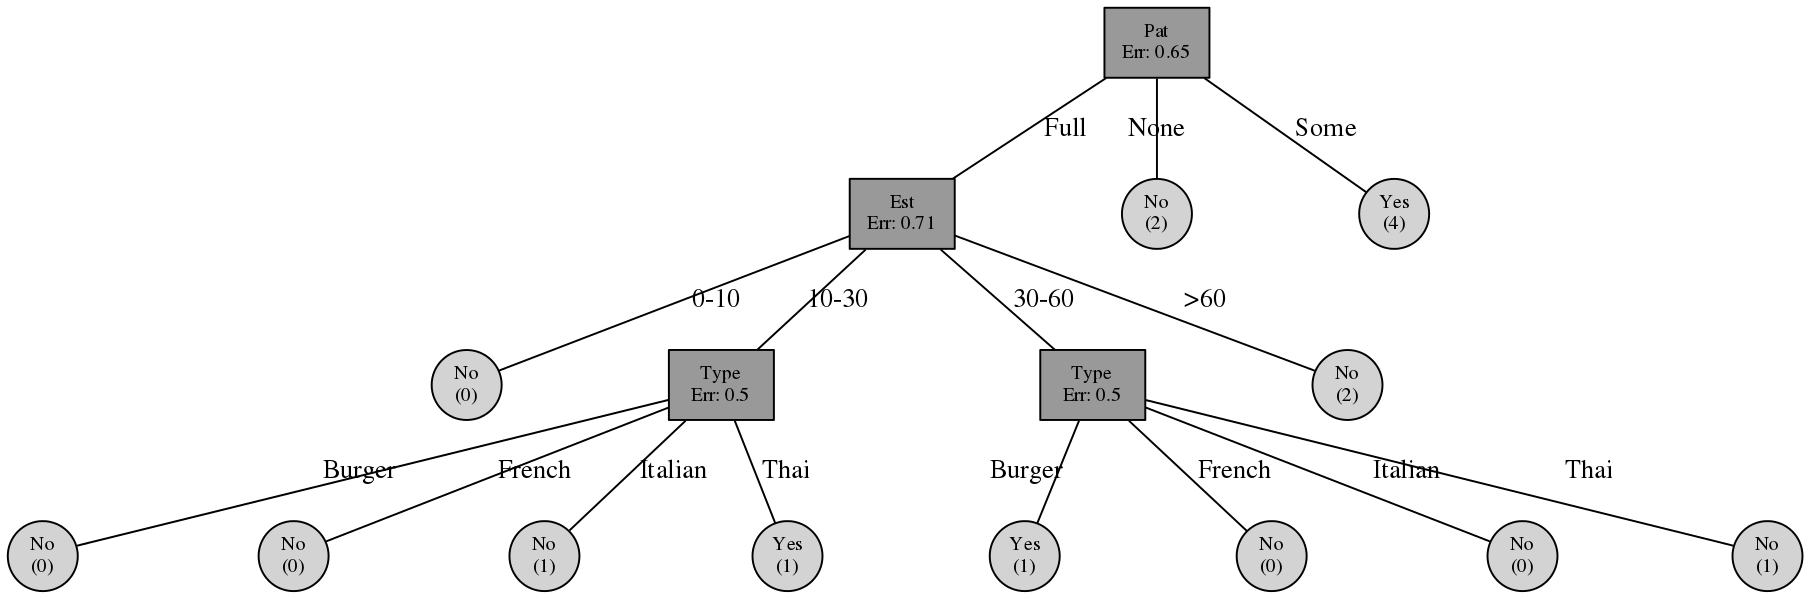
\includegraphics[scale=0.2]{arv1}
    \caption{A árvore para o \texttt{D1}}
    \label{fig:ad1}
  \end{subfigure}
  
  \begin{subfigure}[b]{0.90\textwidth}
    \centering
    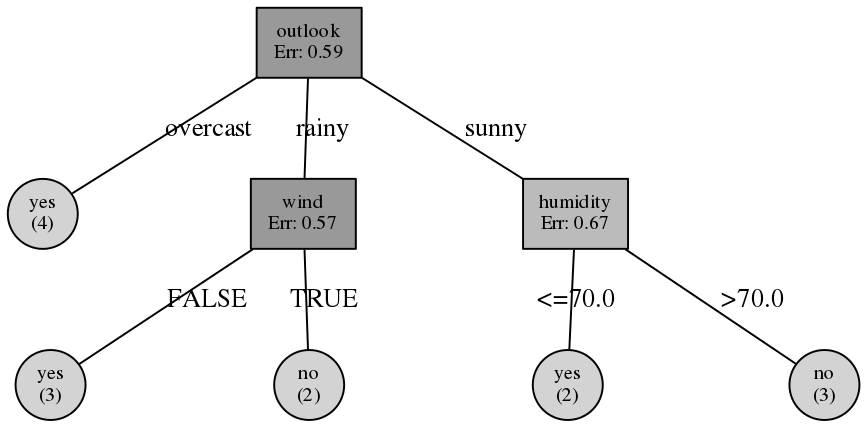
\includegraphics[scale=0.3]{arv2}
    \caption{A árvore para o \texttt{D2}}
    \label{fig:ad2}
  \end{subfigure}

  \begin{subfigure}[b]{0.90\textwidth}
    \centering
    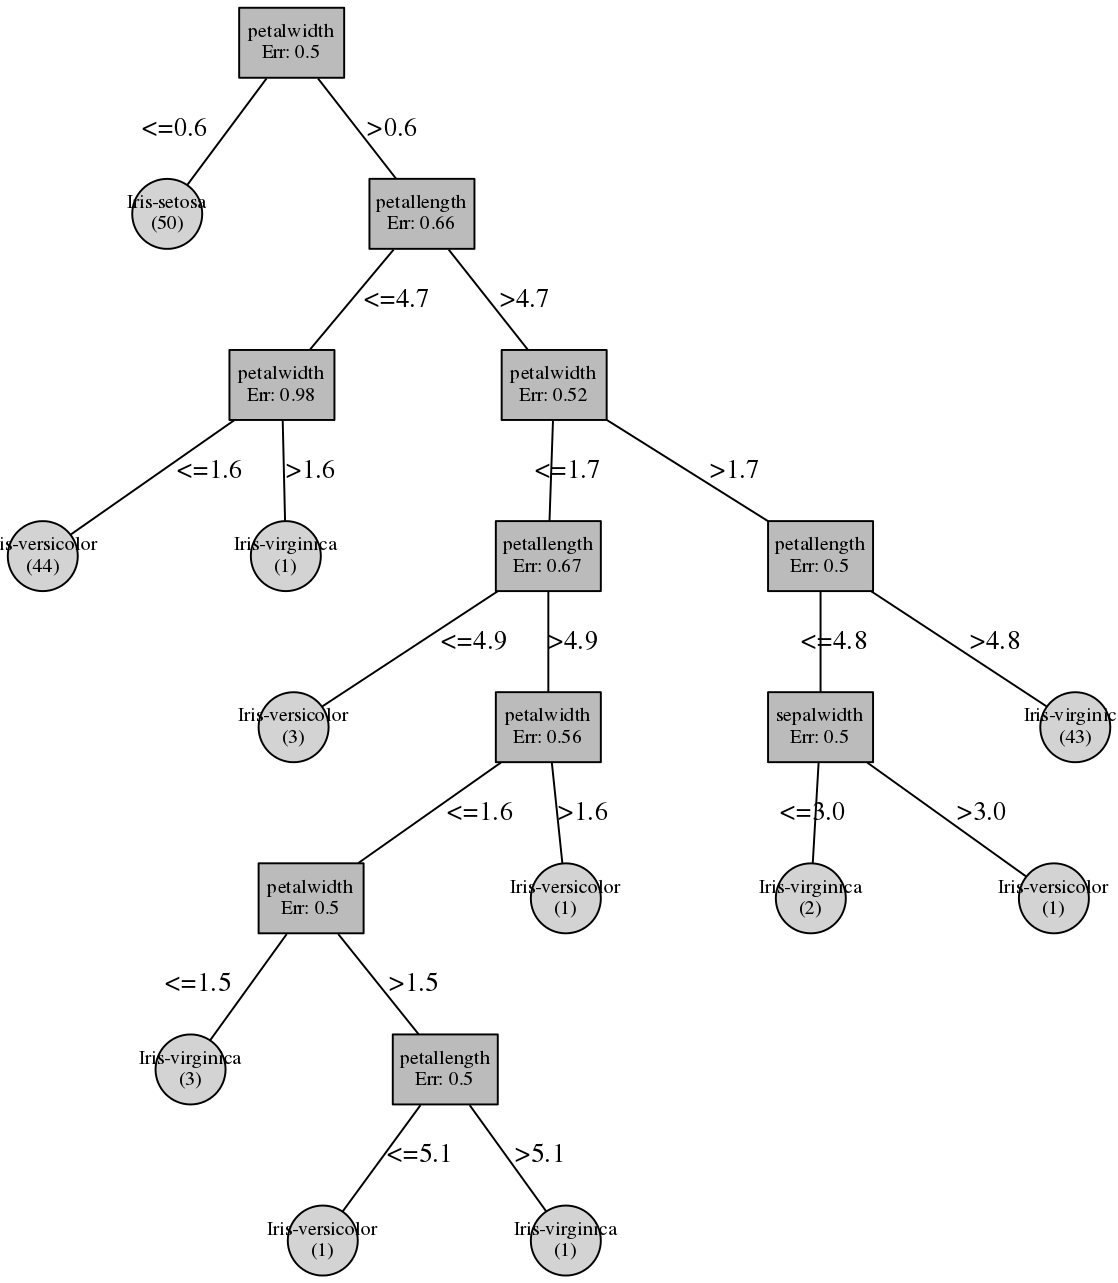
\includegraphics[scale=0.2]{arv3}
    \caption{A árvore para o \texttt{D3}}
    \label{fig:ad3}
  \end{subfigure}
  \caption{Árvores de decisão sem \textit{pruning}}
  \label{fig:anp}
\end{figure}

\lipsum[3]

\lipsum[4]

\lipsum[5]


%----------------------------------------------------------------------------------------
%	SECTION 6
%----------------------------------------------------------------------------------------

\section{Conclusão}
\label{sec:con}

% Falar de outros métodos como boosting, MCMC... como melhorar a nossa
% implementacao: introduzir random, ir buscar a melhor...

\lipsum[0]

\lipsum[1]

\lipsum[2]


\bibliographystyle{plain}
\bibliography{lab_report_4}

\end{document}
